% !TeX spellcheck = it_IT
\newpage
\section{Ingegneria del software sostenibile}
Il digitale aumenta l'impronta ecologica ma può anche contribuire a ridurla rendendo più efficiente l'uso delle risorse.\\
L'\textbf{ingegnere del software} progetta, sviluppa, manutene, testa e valuta prodotti software.\\
L'obiettivo è quello del \textbf{triangolo di ferro}, ovvero coniugare \textbf{tempi}, \textbf{costi} e \textbf{qualità}.

\subsection{Modello GREENSOFT}
\begin{definition}[GREENSOFT]
	Lo sviluppo software secondo il modello GREENSOFT prevede di utilizzare tecniche che permettano di \textbf{monitorare} gli impatti positivi e negativi sull'ambiente durante tutto il ciclo di vita in modo da garantirne l'ottimizzazione.
\end{definition}
\begin{center}
	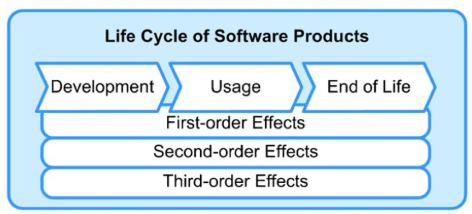
\includegraphics[scale=0.4]{greensoft_1.png}
	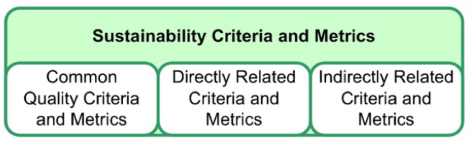
\includegraphics[scale=0.4]{greensoft_2.png}
\end{center}
\begin{center}
	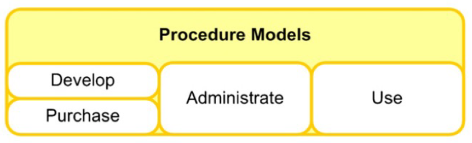
\includegraphics[scale=0.4]{greensoft_3.png}
	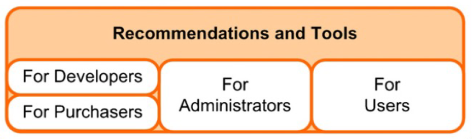
\includegraphics[scale=0.4]{greensoft_4.png}
\end{center}

\begin{center}
	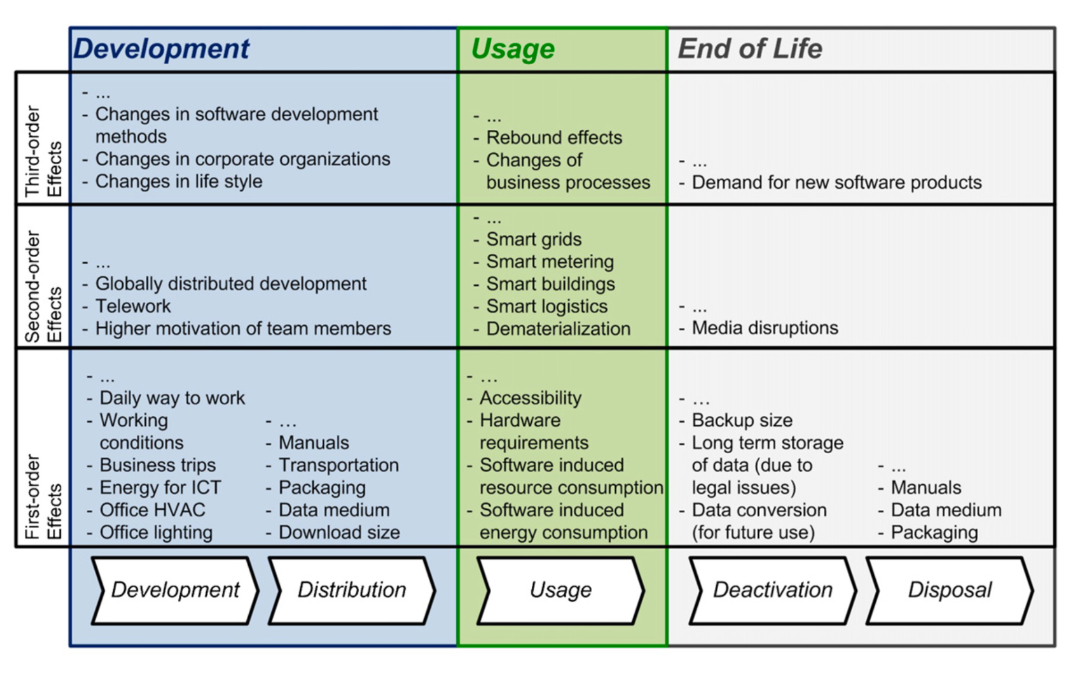
\includegraphics[scale=0.4]{greensoft_lifecycle.png}
\end{center}

\noindent Questa tabella rappresenta le tre categorie principali degli effetti dello sviluppo software sull'ambiente:
\begin{itemize}
	\item \emph{First order}: effetti dovuti alla \textbf{fornitura} di sistemi ICT (Green IT)
	\item \emph{Second order}: effetti dovuti all'\textbf{utilizzo} di sistemi ICT (Green by IT)
	\item \emph{Third order}: effetti \textbf{sistemici} dell'IT (effetto \emph{rebound})
\end{itemize}
che avverrà in maniera \textbf{agile}:
\begin{center}
	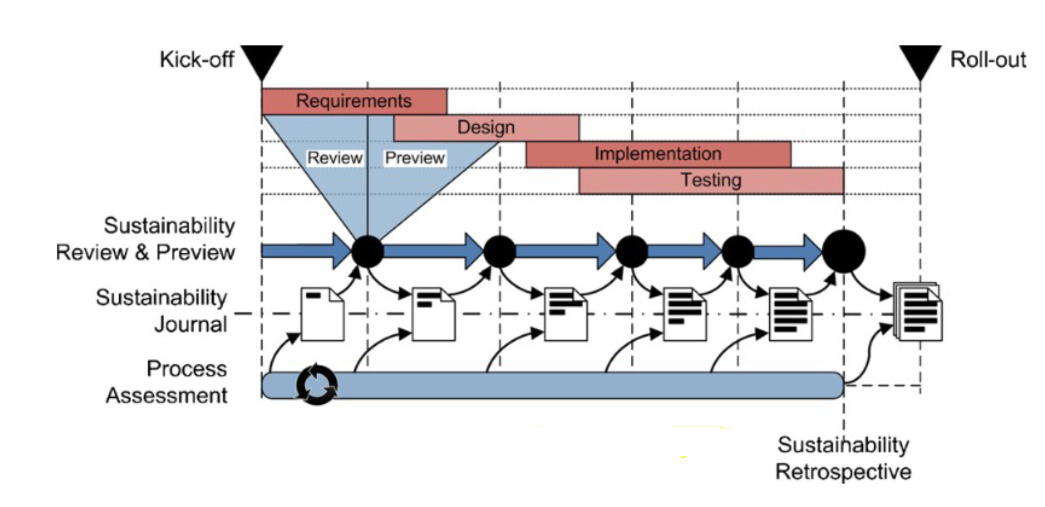
\includegraphics[scale=0.4]{greensoft_agile.png}
\end{center}
\subsection{Principi}
I principi dell'ingegneria del software sostenibile sono i seguenti:
\begin{enumerate}
	\item \textbf{Carbonio}: costruire applicazioni efficienti dal punto di vista del carbonio
	\item \textbf{Elettricità}: costruire applicazioni efficienti dal punto di vista energetico
	\item \textbf{Intensità di carbonio}: consumare elettricità con la minore intensità di carbonio
	\item \textbf{Embodied carbon}: costruire applicazioni efficienti dal punto di vista dell'hardware
	\item \textbf{Proporzionalità energetica}: massimizzare l'efficienza energetica dell'hardware
	\item \textbf{Networking}: ridurre la quantità di dati e la distanza da percorrere nella rete
	\item \textbf{Modellamento della domanda}: costruire applicazioni consapevoli delle emissioni di carbonio
	\item \textbf{Misurazione e ottimizzazione}: ottimizzazioni graduali che aumentino l'efficienza complessiva delle emissioni di carbonio
\end{enumerate}

\subsection{Caso di studio}
Prendiamo come caso di studio gli aggiornamenti di un sistema operativo:
\begin{center}
	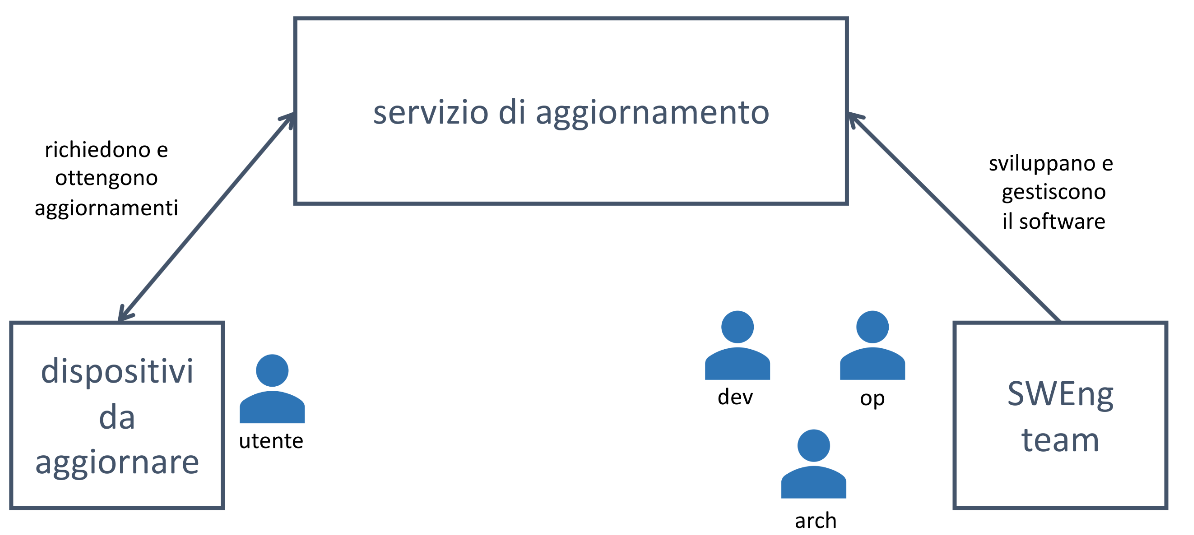
\includegraphics[scale=0.3]{os_update.png}
\end{center}
e analizziamo la situazione sia dal punto di vista dell'\emph{utente} che dello \emph{sviluppatore}.
\subsubsection{Utente}
Supponiamo un aggiornamento di 10 minuti con un consumo medio di $50W$. Abbiamo quindi $50W \cdot \frac{1}{6}h = 8.3 Wh$. Se consideriamo un aggiornamento al mese in un anno abbiamo circa $100W$ per ogni utente, che aumenta molto velocemente se consideriamo ad esempio Windows con un miliardo di utenti.
\begin{equation*}
	0.1kWh \cdot 10^9 = 10^8kWh = 100GWh
\end{equation*}
che corrispondono a $43259$ tonnellate di $CO_2-eq$, ovvero circa ciò che serve per alimentare $5449$ case in un anno.\\
Dal punto di vista dei costi, l'utente non è particolarmente impattato: se assumiamo un costo medio dell'elettricità di $0.3 \frac{€}{kWh}$, un utente ogni anno spenderà $0.03€$ e circa $2h$ di tempo.\\
Cosa può fare?
\begin{itemize}
	\item Essere \textbf{consapevoli} del proprio impatto ambientali
	\item Richiedere software di \textbf{qualità migliore} per evitare patch
	\item Richiedere che la \textbf{sostenibilità} non alteri i requisiti esistenti
\end{itemize}

\subsubsection{Architetto}
Gli architetti sono coloro che determinano i \emph{requisiti funzionali} e non del sistema e che progettano le \emph{interazioni} tra i componenti. Ne l caso di aggiornamenti di un sistema operativo:
\begin{itemize}
	\item \emph{Funzionali}:
	\begin{itemize}
		\item Consegna corretta dell'aggiornamento
	\end{itemize}
	\item \emph{Non funzionali}:
	\begin{itemize}
		\item $99.9\%$ di disponibilità del servizio
		\item Scalabilità
		\item Durata di 10 minuti al massimo tra download e installazione
	\end{itemize}
\end{itemize}
Per rendere gli aggiornamenti più sostenibili gli architetti devono lavorare sui requisiti non funzionali:
\begin{itemize}
	\item \textbf{Scomponendo} i servizi in unità scalabili:
	\begin{itemize}
		\item \textbf{CDN}: mantenere i dati dell'aggiornamento \emph{vicini}, riducendo la \emph{banda} necessaria tramite del \emph{caching}
		\item \textbf{Microservizi}
	\end{itemize}
	\item \textbf{Bin packing}: è una tecnica che cerca di minimizzare il numero di server per far girare i servizi che compongono il sistema
	\item \textbf{Carbon awareness}: ad esempio Windows Update schedula gli aggiornamenti in base alle emissioni di carbonio di dove si trova la macchina e dall'orario
\end{itemize}
\subsubsection{Sviluppatore}
Gli sviluppatori implementano i requisiti specificati dall'architetto ponendo attenzione ad alcune scelte tecniche:
\begin{itemize}
	\item \textbf{Linguaggio} di programmazione: trovare un bilanciamento tra \emph{energia} consumata, \emph{tempo} di esecuzione e \emph{memoria} utilizzata
	\item \textbf{Librerie} con algoritmi efficienti
	\item \textbf{Pattern} efficienti (e.g. \emph{event driven} invece di \emph{polling})
	\item \textbf{Implementative}: favorire \emph{bin packing} e disaccoppiare software da struttura per facilitare la migrazione
\end{itemize}
Il programmatore può fornire \textbf{metriche} con \emph{KPI} che siano rapporti tra quantità, e.g. $\frac{\text{CPU Usage}}{\text{Updates delivered}}$
\subsubsection{Operatore}
L'operatore è colui che \textbf{gestisce} e \textbf{garantisce} la disponibilità dell'applicazione. Deve:
\begin{itemize}
	\item Offrire \textbf{risorse} infrastrutturali adeguate: favorire il \emph{bin packing}
	\item Utilizzare al meglio le risorse per contenere i \textbf{costi} e favorire la \textbf{sostenibilità}, ad esempio con auto-scaling
	\item Garantire \textbf{backup e ripristino} nella giusta quantità
	\item Implementare \textbf{logs} e \textbf{monitoraggio} (KPI infrastrutturali vs KPI aziendali)
\end{itemize}

\subsection{Quadro normativo}
Le leggi e i regolamenti possono favorire  una transizione sostenibile tassando le \textbf{esternalità negative} (emissioni nel lifecycle) e obbligando alla trasparenza.\\
L'Unione Europea ha definito all'interno del Green Deal una direttiva sul \emph{Corporate sustainability reporting} che obbliga le grandi aziende a relazionare sulla loro sostenibilità.\\
A livello globale purtroppo è improbabile che avvenga.